\documentclass{article}%
\usepackage[T1]{fontenc}%
\usepackage[utf8]{inputenc}%
\usepackage{lmodern}%
\usepackage{textcomp}%
\usepackage{lastpage}%
\usepackage[head=40pt,margin=0.5in,bottom=0.6in]{geometry}%
\usepackage{graphicx}%
%
\title{\textbf{Vecinos de San Agustín protestaron por el asesinato de un niño de 12 años}}%
\author{EL NACIONAL WEB}%
\date{11/10/2018}%
%
\begin{document}%
\normalsize%
\maketitle%
\textbf{URL: }%
http://www.el{-}nacional.com/noticias/sociedad/vecinos{-}san{-}agustin{-}protestaron{-}por{-}asesinato{-}nino{-}anos\_255391\newline%
%
\textbf{Periodico: }%
EN, %
ID: %
255391, %
Seccion: %
Sociedad\newline%
%
\textbf{Palabras Claves: }%
NO\_TIENE\newline%
%
\textbf{Derecho: }%
1.1, %
Otros Derechos: %
, %
Sub Derechos: %
1.1.1.9\newline%
%
\textbf{EP: }%
SI\newline%
\newline%
%
\textbf{\textit{El joven fue identificado como Kevin Segovia de 12 años de edad y al momento de su muerte estaba junto a su papa yendo al colegio}}%
\newline%
\newline%
%
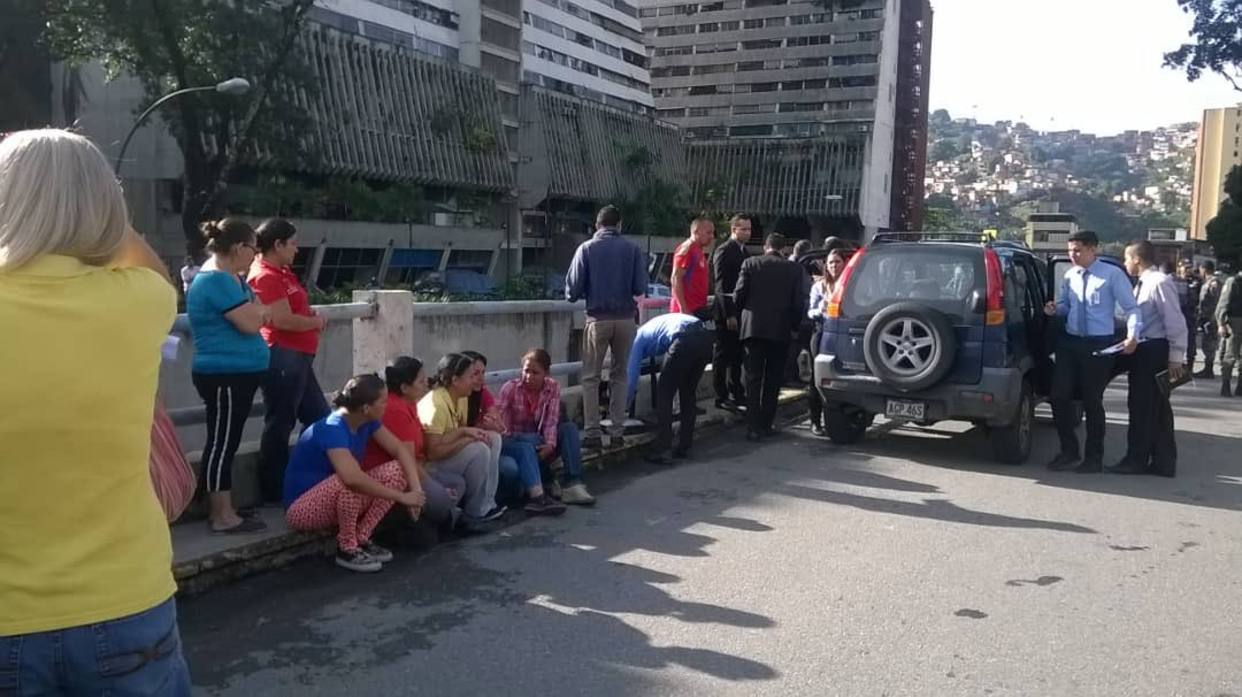
\includegraphics[width=300px]{8.jpg}%
\newline%
%
Ciudadanos de la localidad de San Agustín en Caracas protestaron este jueves en rechazo a la muerte~de un niño de 12 años que recibió un impacto de proyectil en la cabeza tras quedar en el medio de un enfrentamiento entre policías y delincuentes.%
\newline%
%
El joven fue identificado como Kevin Segovia~y al momento de su muerte viajaba con su papá en un vehículo partícular en dirección al colegio del menor,~ubicado en las cercanías del Museo del Niño.%
\newline%
%
“A las 6:50 am inició el tiroteo y varias personas los empezamos a resguardar, mientras estábamos metiendo a los niños a la escuela y vimos al señor trayendo al niño muerto”, dijo una ciudada de la zona para TVVenezuela.%
\newline%
%
\end{document}